\chapter{Numerical Method}
\label{sec:methods}
In the previous chapter, the basics of plasma physics and the mathematical tools required to analyze plasma dynamics were introduced. Solving the equations of motion for the millions of plasma particles analytically is impractical, this section will outline the Particle-in-Cell (PiC) algorithm as a framework for computer simulation of plasma. A method for implementing photoelectron emission from conducting surfaces is emphasized. First, a general description of the PiC algorithm is introduced as well as the stability criteria of the algorithm. Then the implementation of the PiC algorithm in the PINC framework is discussed with emphasis on the implementation of object charging in plasma. Finally, a method for implementing photoelectron emission into the PINC object module is presented.

\section{Particle In Cell algorithm}
The particle in cell algorithm is a method used in computational plasma physics to analyze large systems of many particles in a computationally efficient manner. This is achieved by the introduction of super particles, computational particles, that represent many real particles, then interpolating the forces acting on these super particles to a spatial grid.\\
There are three main ways of simulating the forces acting on a system particles. The particle-particle method (PP) where forces are computed between individual particles. The particle-mesh method (PM) where the forces between the particles are computed as field quantities on the spatial mesh. And the particle-particle-mesh method (PPPM or $P^3M$), which is a combination of the two earlier methods.\\
By far the simplest method computationally is the PP method. However, since all forces between each individual pair of particles are computed, the method is also the most computationally expensive. If the system of interest contains $N_p$ particles, then the number of operations scale as $\mathcal{O}(N^2_p)$ \insertref{Hockney and eastwood p20}. It is therefore impractical to use the PP method for all but the simplest systems, even on highly parallel High Performance Computers (HPC) available today.\\
The PM method computes the forces of a system as field quantities, first by assigning the charges in the system to the mesh by some method, then solving Poisson's equation on the mesh, then computing the forces on the mesh points and interpolating to the individual particles. This method is therefore faster, but usually not as accurate as computing the forces on all particle pairs directly. With $N_g$ grid points, the complexity of this method scales as $\mathcal{O}(N_g \log{N_g})$ thus making this method much more applicable to larger systems than the PP method.

\begin{figure}[h!]
    \centering
    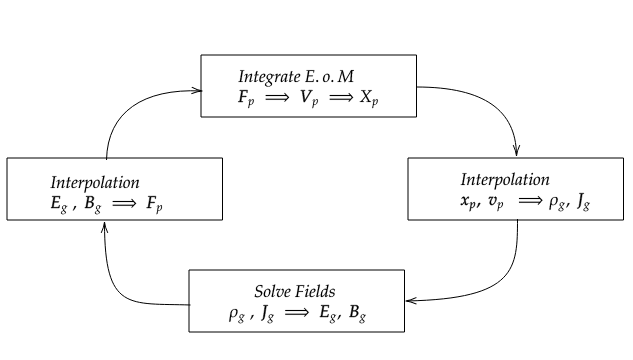
\includegraphics[scale=0.6]{figures/PiC.png}
    \caption{Particle in cell compute cycle}
    \label{fig:pic}
\end{figure}

The PiC algorithm is an example of the PM method, figure \ref{fig:pic} shows an overview of a computational cycle for each time step in the PiC algorithm. Beginning at the box on the right in the figure, a distribution of $N_p$ particles with position $\vb{x}_p$ is interpolated to get the charge $\rho_g$ and current density $\vb{J}_g$ at the surrounding grid points. The two most common methods for this interpolation is the Nearest Grid Point (NGP) scheme, and Cloud in Cell (CIC) scheme.\\
Once the charge and current densities are known on the grid, the next step is to solve for the $\vb{E}$ and $\vb{B}$ fields. This is accomplished by solving Maxwell's equations at the grid points

\begin{subequations}
    \begin{align}
        Gauss's\; Law: \nabla \cdot \vb{E} &= \frac{\rho}{\epsilon_0} \label{eq:gauss} \\
        Gauss's\; Law\; for\; magnetism: \nabla \cdot \vb{B} &= 0 \\
        Maxwell - Faraday's\; equation: \nabla \cross \vb{E} &= - \pdv{\vb{B}}{t}\\
        Ampere's\; Law: \nabla \cross \vb{B} &= \mu_0 \left(\vb{J} + \epsilon_0 \pdv{\vb{E}}{t} \right)
    \end{align}
\end{subequations}

Where $\rho$ is the charge density, $\epsilon_0$ is the vacuum permittivity, $\mu_0$ is the vacuum permeability, and $\vb{E}$ and $\vb{B}$ are the electric and magnetic fields respectively. With the electric and magnetic field computed at the grid nodes, the force on each super particle is computed from Lorentz's force equation and interpolating back to the position of the super particles. Using some numerical integrator the new position and velocity of the super particle is updated from the computed forces, and the cycle can then be repeated for the next time step. 

\section{Particle in Cell implementation in PINC}
In this section, we discuss the methods implemented in PINC that are required for the main PiC compute cycle described in figure \ref{fig:pic} with focus on the particular schemes used in this thesis. The scheme used in PINC for integrating the equations of motion are presented, followed by the multigrid field solver, and finally the particle weighting scheme is discussed. PINC is the work of many researchers, but have been mainly implemented by Sigvald Marholm as part of his Ph.D thesis \insertref{Sigvald's thesis}, Gullik Killie \insertref{Gullik's thesis}, and Steffen Brask \insertref{Steffen's thesis}. Significant contributions have also been made by Jan Deca, who implemented the module for object charging in PINC. This module will be discussed in more detail later in this chapter. 

\subsection{Integration of the equations of motion}
Planet Mercury possesses and internal magnetic field, as such the plasma surrounding the planet is magnetized. To solve for the motion of magnetized plasma, the Boris algorithm is used to integrate the equations of motion. The Boris algorithm is a variant of the well known leapfrog method, in which the position and velocity of a particle is updated at half time steps in staggered fashion. Like the leapfrog method, the Boris algorithm is an energy conserving integrator; the merits of the Boris algorithm as the de facto particle mover is further expanded upon in the work by Qin et al. \insertref{Why is Boris algorithm so good?}
\\
Using the same notation as defined in \insertref{Plasma physics via computer simulation} the Lorentz force is discretized as 

\begin{subequations}
    \begin{align}
        \frac{\vb{x}^{t+\Delta t}_p - \vb{x}^t_p}{\Delta t} &= \vb{v}^{t + \frac{\Delta t}{2}} \\
        \frac{\vb{v}^{t+\Delta t}_p - \vb{v}^{t-\Delta t}_p}{\Delta t} &= \frac{q_s}{m_s} \left(\vb{E}_p + \frac{\vb{v}^{t+\Delta t}_p - \vb{v}^{t-\Delta t}_p}{2} \cross \vb{B}_p \right) \label{eq:borizVel}
    \end{align}
\end{subequations}

In the Boris algorithm equation \ref{eq:borizVel} is decomposed into a series of updating steps. First, half the acceleration is added, then the intermediary velocity vector is rotated due to the external magnetic field $\vb{B}$, and finally the second half of the acceleration is added.

\begin{subequations}\label{eq:borisNewVel}
    \begin{align}
        \vb{v}^{-} &= \vb{v}^{t-\Delta t}_p + \frac{q_s}{m_s} \vb{E}_p \frac{\Delta t}{2} \\
        \vb{v}^{'}_p &= \vb{v}^{-}_p + \vb{v}^{-}_p \cross \vb{T} \\
        \vb{v}^{+}_p &= \vb{v}^{-}_p + \vb{v}^{'}_p \cross \vb{S} \\
        \vb{x}^{t+\Delta t}_p &= \vb{v}^{+}_p + \frac{q_s}{m_s} \vb{E}_p \frac{\Delta t}{2} 
    \end{align}
\end{subequations}

Where the rotational parameters $\vb{T}$ and $\vb{S}$ are expressed as

\begin{subequations}\label{eq:BrotParams}
    \begin{align}
        \vb{T} &= \hat{\vb{B}}_p \cdot \tan\left(\frac{q_s \Delta t}{2m} B_p \right) \\
        \vb{S} &= \frac{2 \vb{T}}{1 + \vb{T}^2} 
    \end{align}
\end{subequations}

Equations \ref{eq:borisNewVel} are equally suited for plasmas with time varying magnetic fields as for electrostatic plasma with a constant external magnetic field. Since PINC is an electrostatic model, equations \ref{eq:BrotParams} is solved once before the main time loop, then applied to each call to the mover method.

\subsection{Field Solver}
Several field solvers exists in PINC, in this thesis the multigrid solver developed by Vetvik \insertref{Gullik's thesis} has been used. The multigrid solver is an iterative method; the basic principle of the method in a PiC context is to solve Poisson's equation first on a coarse grid, then using the solution on the course grid as a guess, solve the equation again for a finer grid. The solution for the coarse grid speeds up the solution for the finer grid, reducing the total computational time required to converge to an accurate solution. 
\\
There are three main types of multigrid solver, divided into the so called V-cycle, W-cycle and F-cycle, defined by when the algorithm should use a coarser or finer mesh than used in the previous iteration. Multigrid solvers are highly flexible, and many researchers have spent considerable effort in order to optimize the number of iterations \insertref{Killie thesis}, \insertref{Multigrid, Trottenberg et al}, highly optimized multigrid solvers have a local complexity given by $\mathcal{O}(N_g)$, with a global complexity of $\mathcal{O}(N_g log(N_g))$ when using domain decomposition like in the case of PINC \insertref{Steffen's thesis}.
\\
As described earlier, the multigrid method solves Poisson's equation in PINC. Strictly speaking, the solution to Gauss's law, equation \ref{eq:gauss} is solved. In PINC however, electrostatic plasma is assumed, in this case the electric field is irrotational, i.e. $\nabla \cross \vb{E} = 0$ and the electric field can then be represented as the gradient of a scalar potential field $\vb{E} = \nabla \phi$.  Substituting the potential field back into Gauss's law, equation \ref{eq:gauss} we have Poisson's equation

\begin{equation}\label{eq:poisson}
    \nabla^2 \phi = \frac{\rho}{\epsilon}
\end{equation}

In PINC this equation is solved iteratively using the Gauss-seidel method. Gauss-Seidel discretizes \ref{eq:poisson} using the Forward-Time Central-Space (FTCS) finite difference scheme. In one spatial dimension, the electric field in terms of the potential becomes

\begin{equation}\label{eq:Ediscrete}
    \vb{E}_g = \frac{\phi^{n+1}_g - \phi^{n-1}_g}{2\Delta x}
\end{equation}

and Poisson's equation, equation \ref{eq:poisson}, becomes

\begin{equation}\label{eq:poissonDescrete}
    \frac{\phi^{n+1}_g - 2\phi^n_g + \phi^{n-1}_g}{{\Delta x}^2} = - \frac{\rho_g}{\epsilon}
\end{equation}


Where the subscript g implies the evaluation of $\phi$ at grid points, and the superscript p denotes the grid node index. Analogous expressions can be formed in two and three spatial dimensions.

\subsection{Particle weighting}
In the particle in cell method particles can exist anywhere in the continuous spatial computational domain, but forces and charge densities are calculated at discrete grid points \ref{fig:pic} \insertref{Birdsall Ch 2.6}.  Historically, the NGP method and CIC method are used to weight computational particles to the grid. Higher order schemes exists, such as Quadratic Splines (QS) and Cubic Splines (CS), see \insertref{Okuda, SPLINES AND HIGH ORDER INTERPOLATIONS IN PLASMA SIMULATIONS} for an overview on the usage of higher order weighting schemes in plasma simulation. In PINC the CIC method is used; using similar notation as Verboncoeur in his paper \insertref{Particle simulation of plasmas: review and
advances} the weighting function is defined as 

\begin{equation}\label{eq:weightFunc}
    \vb{w}_{i,j,k} = \vb{x}_p - \vb{X}_{i,j,k}
\end{equation}

Where $\vb{x}_p$ is the position of particle p, and $\vb{X}_{i,j,k}$ is the position of the nearest grid point closest to the origin. Using equation \ref{eq:weightFunc}, the charge distribution of particle p to a two dimensional grid can be found as

\begin{subequations}
    \begin{align*}
        Q_{i,j} &= q_p \, (1 - w_i) \, (1 - w_j) \\
        Q_{i+1,j} &= q_p \, w_i \, (1 - w_j) \\
        Q_{i,j+1} &= q_p \, (1 - w_i) \, w_j \\
        Q_{i+1,j+1} &= q_p \, w_i \, w_j 
    \end{align*}
\end{subequations}

With similar equations for the three dimensional case can be found from equation \ref{eq:weightFunc}. From the charge distribution found above, the charge density can be found directly by dividing the charge distribution by the volume of a computational cell, i.e 

\begin{equation*}
    \rho_{i,j,k} = \frac{Q_{i,j,k}}{V_{i,j,k}}
\end{equation*}

From the charge density and current density, PINC computes the electric and magnetic field using the multigrid field solver module.

\section{Simulation stability and constraints}

\subsection{Spatial resolution}
In PINC, and in other particle in cell codes, particles move in continuous space, but their macroscopic properties are projected to a discrete grid. Representing continuous variables on a discrete grid leads to numerical instability called finite grid instability \insertref{Particle simulations of space weather, lapenta 2011, sec 5.1.}. The analysis of finite grid instability is beyond the scope of this thesis, a rigorous mathematical description of finite grid instability can be found in \insertref{Birdsall and Langdon}. The most important result of these analyses is that the grid spacing $\Delta x$ must satisfy the condition

\begin{equation}\label{eq:GridSize}
    \frac{\Delta x}{\lambda_D} < C
\end{equation}


Where C is some constant dependent on the discretization scheme used. In the case of the CIC scheme, the constant C is approximately equal to $\pi$. Failure to meet this condition in a PIC simulation leads to unphysical heating of the plasma. Equation \ref{eq:GridSize} must therefore be satisfied in all directions of the full computational domain to ensure conservation of energy.

\subsection{temporal resolution}
In PINC, the boris algorithm is used for particle pushing. The boris algorithm is an explicit forward time integration scheme, and as such simulations run with PINC must satisfy temporal stability constraints associated with such schemes. In \insertref{hockey and eastwood} and \insertref{birdsall and langdon} and \insertref{lapenta, 2011} a Von Neumann stability analysis of a harmonic oscillator without an external magnetic field given by the following equation

\begin{equation}\label{eq:harmonicOscillator}
    \frac{q_s}{m_s} \vb{E}_p(\vb{x}_p) = - \Omega^2 \vb{x}_p
\end{equation}

leads to the equation 

\begin{equation}
    \left(\frac{\Omega \Delta t}{2} \right)^2 = \sin^2{\left(\frac{\omega_N \Delta t}{2}\right)}
\end{equation}

Where $\omega_N$ is the numerical oscillation frequency. For values outside the range [-1,1] the sine function has only complex solutions, thus for time steps $\Delta t$ where  $\Omega \Delta t > 2$ is true, the numerical oscillation frequency will be complex. Any practical simulation of the harmonic oscillator will therefore become unstable due to unbounded numerical heating. Thus, the finite time stability criteria can be expressed as

\begin{equation}
    \Omega \Delta t < 2
\end{equation}

In this thesis, for solar wind simulations, the frequency $\Omega$ that needs to be resolved is typically the electron oscillation frequency of the cold solar wind plasma. 


\subsection{The CFL condition}
The Courant–Friedrichs–Lewy condition, or CFL condition, is a stability criteria linking the finite time step and grid step, $\Delta t$ and $\Delta x$ respectively. The condition must be met everywhere in the computational domain if the explicit integrator in PINC is to converge to a solution.

In \insertref{See Steffens master thesis..} a common formulation of the condition is given as

\begin{equation}
    \frac{\Delta x}{\Delta t} > C
\end{equation}

Where C is some characteristic speed. The constant C is solver scheme dependent, and is often set as $C = 1$ for explicit schemes; in PINC this qualitatively means that a particle is restricted to move by maximum one computational cell per time step as the length scale is normalized to the grid step size.

\section{The PINC Object module}
The object module in PINC contains a set of functions and data structures necessary for simulating objects immersed in plasma. It was developed primarily by Jan Deca, and Sigvald Marholm as a part of a collaboration between the University of Oslo and University of Colorado Boulder. In the object module, spacecraft-plasma interations are simulated using the same Capacitance Matrix method outlined by Miyake and Usui in developing the PIC code EMSES (the ElectroMagnetic Spacecraft Environment Simulator) \insertref{New electromagnetic particle simulation code for the analysis of spacecraft-plasma interactions}. 

In this section the method used in PINC for defining objects on a structured Cartesian grid is discussed in brief; a description of the \textit{Grid} data structure and associated functions in PINC is also introduced as all scalar and vector fields are represented in PINC using this data structure, including conducting objects which are defined as scalar fields. The capacitance matrix method is then outlined, with an emphasis on the equations that have been implemented in PINC. 



\subsection{Representing objects on a grid}
In the PINC object module, conducting objects are represented as points on the Cartesian computational grid, and stored in an input HDF5 (Hierarchical Data Format) file. Internally in PINC, this file is converted to a PINC \textit{Grid} structure instance and is stored as a subset of the \textit{Object} data structure which additionally contains data on which nodes are internal to the object, which nodes are on the surface, and data required in photoemission computations. Required data for photoemission in the \textit{Object} structure will be described in the later section on implementation of photoemission in PINC.

The PINC \textit{Grid} structure is a generalized data structure that stores N-dimensional data in a flat manner. The values on the grid is stored in a lexicographical manner; the elements of the three dimensional array is then represented in PINC as

\begin{equation*}
    (0,0,0), \, (1,0,0), \,, \, (2,0,0), \, ... \, , \, (0,1,0) \,, \, (1,1,0) \,, \, (2,1,0) \,, \, ...
\end{equation*}

Objects in PINC are thus stored as 1 by N arrays representing scalar fields, where N is the total number of grid points in the computational domain. The \textit{Grid} structure additionally contains a data field called \textit{sizeProd}, that allows for converting between Cartesian grid point coordinates and the index of value in the array: This field is an array that contains the cumulative product of the number of grid points along each axis in the computational domain. Thus, the index $p$ of the value of a \textit{Grid} structure located at the Cartesian coordinates $(x,y,z)$ is represented as

\begin{equation}\label{eq:PINCindex}
    p = x \cdot \text{sizeProd}[0] + y \cdot \text{sizeProd}[1] + z \cdot \text{sizeProd}[2]
\end{equation}

Traversing along an axis from a point with index $p$ of the \textit{Grid} structure, is then the simple matter of adding the corresponding element of the \textit{sizeProd} array to the index $p$. We will make use of this fact, along with equation \ref{eq:PINCindex}, later in this chapter in creating an algorithm for photoemission on the surface of conducting objects. 


\subsection{The capacitance matrix method}
The general idea of the capacitance matrix method is to precalculate a capacitance matrix for each object immersed in the plasma in question. Applying the computed capacitance matrix, the charges due to super-particles impinging the object can be redistributed to the surface of the object, after redistribution of charges a charge density and electric potential correction is computed and spacecraft potential can be updated. super-particles located within the object are then removed from the computational domain after their charges have been redistributed. 

\todo{Create a new cycle diagram}
Figure \insertref{Updated PIC cycle diagram} shows a modified computational cycle for PINC when taking into account charge accumulation on the surface of a conducting object immersed in the plasma.

The capacitance matrix relates the potential $\phi$ and charge distribution $\rho$ as follows \insertref{New electromagnetic particle simulation code for the analysis of spacecraft-plasma interactions}

\begin{equation}
    \rho_i = \sum^{N_G}_{j=1} A_{ij} \phi_j
\end{equation}

Where the matrix A represents the capacitance matrix, where i and j are the indices of the grid, and $N_G$ is the total number of grid points. Inverting matrix A, and defining $B \equiv A^{-1}$, the potential $\phi$ can be calculated as 

\begin{equation}
    \phi_i = \sum^{N_G}_{j=1} B_{ij} \rho_j
\end{equation}


After redistribution of charges, the charge density on the conducting body surface $\rho_s$ changes. The correction in potential on the spacecraft surface $\delta \phi_s$ can then be found from the charge density correction $\delta \rho_s$ as

\begin{equation}
    \delta \phi_{s,i} = \sum^{N_B}_{j=1} B_{ij} \delta \rho_{s,j}
\end{equation}

Where $N_B$ is the total number of surface nodes, and $N_B < N_G$. By forming a subset of matrix B with the values associated with the surface nodes, with $N_B$ rows and columns, and inverting this matrix the charge density correction on the surface can be found

\begin{equation}\label{eq:SCchargeCorr}
    \delta \rho_{s,i} = \sum^{N_B}_{j=1} C_{ij} \delta \phi_{s,j}
\end{equation}

Where the matrix $C$ is the inverted sub matrix of B. Qualitatively $C$ is the capacitance matrix of the conducting surface. In the PINC object module, matrix $C$ is constructed and stored before the main simulation loop begins by placing a unit charge on each grid point defining the conducting object surface, setting all other grid points to zero charge, and then solving for the potential: This forms the sub matrix of matrix $B$ which can then be inverted to find the surface capacitance matrix $C$, details of this implementation are found in appendix \ref{sec:ObjectCode}.

In the simulation time-loop of PINC, after the potential has been updated, but before charges have been distributed to the surface, the surface potential of the conducting body $\phi_{s,j}$ is not the same value for all values of j and is therefore not at an equipotential. 

The correction in potential in terms of the equipotential $\phi_C$ of the surface is given by

\begin{equation}\label{eq:SCphiCorrEqui}
    \delta \phi_{s,j} = \phi_C - \phi_{s,j}
\end{equation}

Substituting equation \ref{eq:SCphiCorrEqui} into equation \ref{eq:SCchargeCorr}, the charge density correction equation becomes

\begin{equation}\label{eq:SCrhoCorrNew}
    \delta \rho_{s,i} = \sum^{N_B}_{j=1} C_{ij} (\phi_C - \phi_{s,j})
\end{equation}

The equipotential $\phi_C$ is unknown in equation \ref{eq:SCrhoCorrNew}; by using the fact that charges must be conserved when impinged charges are redistributed to the object surface, the equipotential can be calculated. Conservation of charge takes the form

\begin{equation}\label{eq:ConsSurfCharge}
    \sum^{N_B}_{i=1} \delta \rho_{s,i} = 0
\end{equation}

Substituting equation \ref{eq:SCrhoCorrNew} into equation \ref{eq:ConsSurfCharge}, $\phi_C$ can be computed as

\begin{equation}\label{eq:Equipotential}
    \phi_C = \frac{\sum_i \sum_j C_{ij} \phi_{s,j}}{\sum_i \sum_j C_{ij}}
\end{equation}

In the conducting object run mode of PINC, after a first pass of the multigrid Poisson solver, equations \ref{eq:SCrhoCorrNew} and equation \ref{eq:Equipotential} are solved to redistribute absorbed charged particles, a new pass with the Poisson solver then solves the new potential field using the correction to the charge density field. Details on the implementation of these equations in PINC can be referenced by contacting the 4DSpace group at the University of Oslo for access to the PINC code repository.

\newpage

\section{Implementing photoemission in PINC}

Photoelectric emission by sunlit spacecraft surfaces contribute significantly to the overall charge of a spacecraft. In fact, in normal conditions in geosynchronous orbits, the photoelectron flux exceeds that of the ambient electrons \insertref{Aspects of spacecraft charging in sunlight}. When there is a net outgoing current flux, spacecraft charge to to a positive voltage. In order to simulate spacecraft charging using PINC, it is then necessary to implement photoelectric emission. In this section the photoemission method implemented as part of this thesis is presented. 


\begin{figure}[h!]
    \centering
    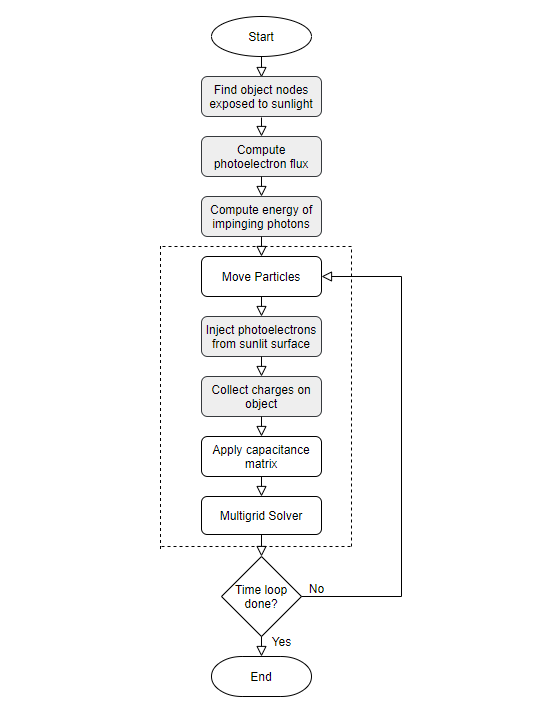
\includegraphics[width=12
    cm, height=15cm]{figures/photoemission.PNG}
    \caption{Flowchart describing the photoemission algorithm}
    \label{fig:photoemission}
\end{figure}

The flowchart shown in figure \ref{fig:photoemission} describes the general flow of PIC method as implemented in PINC when the photoemission modules developed for this thesis are included. Processes shown in the diagram are on a function level in the code, with processes colored grey describing functionality that needed to be implemented in PINC. The details of the implementation of these processes are shown later in this section. The functions placed within the stippled box are carried out for each iteration of the PIC time loop; since these functions are called with a greater frequency, it is vital that they are computationally efficient.

In addition to the functions described in the figure \ref{fig:photoemission}, the initialization function of the object structure in PINC was expanded to read input parameters required for the new photoemission functions. To facilitate ease of use, and to make the code more easily readable, function pointers were added such that the functions for computing photoelectron flux and photoelectron injection could be specified as part of an input file. 


\subsection{Finding object nodes exposed to sunlight}

To be able to simulate photoemission our code needs to know what surfaces the photoelectrons are supposed to be emitted from. As discussed in the previous section on the PINC object module, PINC has no "knowledge" on what faces make up the surface of an object embedded in the computational domain. Thus, it is necessary to locate the object nodes that are exposed to direct sunlight.

The two functions developed to find these surface nodes are directly linked to the functions that inject photoelectrons into the computational domain since a more complex function is required to find the subset of surface nodes used to fill computational cells adjacent to the sunlit object surface. 

The general method for finding the sunlit surface nodes is fairly straight forward, and has been programmed with the assumption that photons travel in the same direction as the x axis of the domain to reduce the complexity of the code. 

Beginning at the node with index 0 of the domain, the code steps along the x direction checking whether each node index is an element of the array containing all object surface nodes. When the node index matches the index of a surface node, the index is stored in the object structure, and the loop stepping along the x axis is exited. The loop of stepping down the x axis is then repeated for each node along the y and z axis until the function has iterated through each "column" normal to the YZ plane. If a surface node is not located in a column parallel to the x axis, the function simply continues to the next column.

This function can be visualized as analogous to mapping the topology of the bottom of a lake by sinking a weight attached to a rope from the surface of the lake, and measuring the wetted length of the rope when the weight reaches the bottom.


\begin{minipage}{\linewidth}
\begin{lstlisting}[language=C, caption={Pseudo code for finding sunlit object surface nodes},
                    label={lst:sunlitNodes}]
void oFindAllSunlitNodes(...){

    ... define and initialize variables ...

    for(int k = 0; k<size[z]; k++){
    
        for(int j = 0; j<size[y]; j++){
                
            int flag = 0;
            for(int i = 0; i<size[x]; i++){
                
                index = i*sizeProd[1] + j*sizeProd[2] + k*sizeProd[3];
                for(int n = 0; n < nSurfaceNodes; n++){
                    
                    surfNode = surface[n];
                    if(surfNode == index){
                        ... append index to exposed node array ...
                        flag = 1;
                        break;
                    }
                    
                if(flag) break;
                
                }
            }
        }
    }
}
\end{lstlisting}
\end{minipage}

\vspace{1cm}
Listing \ref{lst:sunlitNodes} shows the basic structure of the function described above, each column normal to the YZ plane is stepped down using the "size" array that stores the number of nodes along each axis of the domain. The index is then found using equation \ref{eq:PINCindex} and compared with the indices of surface nodes stored in the "surface" array. The surface array is initialized by the function that computes the object capacitance matrix, which is called before the sunlit surface nodes are found. In the photoelectron injection function, the indices of the sunlit nodes can then be converted into Cartesian coordinates with a helper function using the "sizeProd" array. 

A similar function to listing \ref{lst:sunlitNodes} finds the subset of sunlit object nodes that are used for photoelectron injection by filling cells adjacent to the emitting surfaces.
Since PINC does not store data defining cells, we choose the cell to be filled by the vertices $[i-1,j,k], [i-1,j+1,k], [i-1,j,k+1], [i-1,j+1,k+1], [i,j,k], [i,j+1,k], [i,j,k+1], [i,j+1,k+1]$. In PINC we have defined the sunlit surface of the object by the projection of the object onto the YZ plane, therefore for a cell to be "on" the surface of the object we require that the vertices $[i,j,k], [i,j+1,k], [i,j,k+1], [i,j+1,k+1]$ of the cell are also surface nodes.

\begin{figure}[h!]
    \centering
    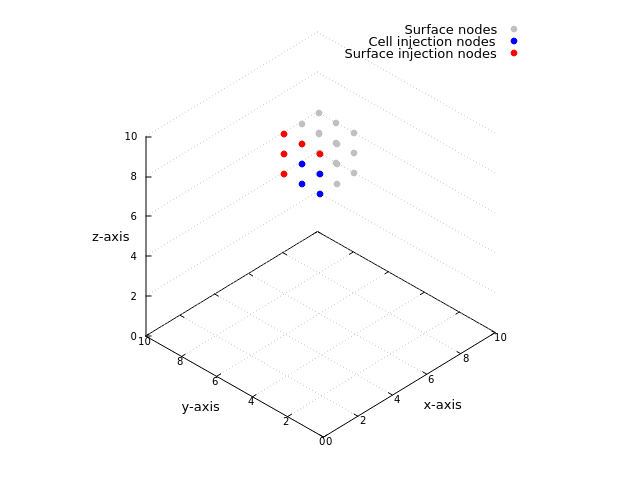
\includegraphics[scale=0.6]{figures/nodes.png}
    \caption{Surface nodes on a box exposed to sunlight}
    \label{fig:sunlitNodes}
\end{figure}

Figure \ref{fig:sunlitNodes} shows the surface nodes of a 2 unit by 2 unit box,


\subsection{Integrating Planck's law}

As discussed in the theoretical background, the photoelectron flux is dependent on the material composition of the sunlit surface. Surfaces with a lower work function tend to eject more photoelectrons. Similarly, the photoelectron flux of a sunlit surface is proportional to the distance from the surface to the sun. Since the power output of the sun follows an inverse square law with the square of the distance from the sun, the closer the spacecraft is to the sun in its orbit the higher amount of photons above the work function strike the surface of the spacecraft. Both these factors need to be accounted for in order to make the simulation of spacecraft charging in sunlight as general as possible. 
Thus, to compute the photoelectron flux for a particular spacecraft, Planck's law must be integrated in the frequency band from the work function frequency, to infinity before the main particle-in-cell loop is started. The photoelectron flux can then be directly computed from the power output received by the spacecraft, as long as the surface area exposed to the sun and work function of the spacecraft material surface is known. These variables can given as input to our simulation. Additionally, integrating Planck's law allows the average kinetic energy of the emitted photoelectron to be calculated, simply by dividing the total radiation energy absorbed per timestep by the total photoelectron flux.
Several methods for numerically integrating Planck's law efficiently exists. In this thesis, the method settled on is based on the paper by Widger and Woodall \insertref{Integration of the Planck Blackbody Radiation Function}. A summary of the method presented in that paper, and the implementation in PINC as C code will now be given.

First, to simplify the integrals, Planck's law is recast in terms of the wavenumber ($cm^{-1}$) $\nu$ rather than frequency of radiation. Planck's law then takes the form

\begin{equation}\label{eq:PlanckNu}
    B(T) = C_1 \int^{\infty}_{\nu} \nu^3 \left(\exp{\frac{C_2 \nu}{T}} - 1 \right) d \nu
\end{equation}

Where B(T) is the radiance, given in units of $W cm^{-2} Sr^{-1}$, T is the absolute temperature in Kelvins, and $C_1$ and $C_2$ are the first and second radiation constants respectively.

Letting $x = C_2 T^{-1} \nu$, equation \ref{eq:PlanckNu} can be rewritten as 

\begin{equation}\label{eq:PlanckX}
    B(T) = C_1 C_2^{-4} T^4 \int^{\infty}_x \frac{x^3}{\exp{x} - 1} dx
\end{equation}

The integrand in equation \ref{eq:PlanckX} can be expanded in a series form, substituting that series into equation \ref{eq:PlanckX} and integrating by parts, equation \ref{eq:planckX} becomes

\begin{equation}\label{eq:PlanckSum}
    \int^{\infty}_x \frac{x^3}{\exp{x} - 1} dx = \sum^{\infty}_{n=1} \exp{-n x} \left(x^2 n^{-1} + 3 x^2 n^{-2} + 6 x n^{-3} + 6 n^{-4} \right)
\end{equation}

$C_1$, $C_2$ and T are known constants in equation \ref{eq:PlanckX}, and the infinite sum in equation \ref{eq:PlanckSum} is straight forward to compute to some finite tolerance using a C function. The integral in \ref{eq:PlanckSum} is computed in units of radiance $W m^2 Sr^{-1}$, the solid angle $\Omega$ of the photoemitting object with respect to the sun can be calculated as

\begin{equation*}
    \Omega = \frac{A_s}{r^2}
\end{equation*}

Where $A_s$ is the area of the sunlit surface, and $r$ is the radial distance from the center of the sun to the object. Multiplying the result of \ref{eq:PlanckSum} by the solid angle of the object with respect to the sun, and the surface area of the sun, the power output in the frequency band above the work function of interest can be found. A similar integral to the one found in equation \ref{eq:PlanckSum} can be constructed in terms of photons per second instead of Watts.

Computing the photons impinging on the surface per timestep does not however correspond to the amount of photoelectrons emitted by the sunlit surface. To compute the total photoelectron flux, the photon impinging rate must be multiplied by the surface material reflectance, and the photoelectron yield (number of electrons emitted per incoming photon above the work function of the material) as described in chapter \ref{sec:theory}.

%\subsection{Initialization and normalization of photoelectric flux}

\subsection{Injection of photoelectrons}
The method selected for injecting a Maxwellian velocity distribution of electrons affect the accuracy of the results from a particle in cell simulation. Once the average kinetic energy of the photoelectrons has been calculated as seen in previous sections, a Maxwellian velocity distribution can be constructed from the average velocity. 

The position of the particles must also be distributed into the computational domain in such a way that the particles remain Maxwellian in their velocity distribution. Describing an accurate particle distribution function $f(\vb{x}, \vb{v}, t)$ is especially important for simulations with timescales longer than that that of the ion transit time, and for simulations that include Monte Carlo collision modules \insertref{Loading and Injection of Maxwellian Distributions in Particle Simulations}.  

In the code developed for this thesis, three methods for injecting photoelectrons were analyzed; two methods based on injecting electrons directly from the surface nodes exposed to sunlight, and one method in which electrons were uniformly distributed in the computational cells adjacent to the emitting surfaces.

Later in this chapter, these injection algorithms are tested against the charging simulations of the Solar Probe plus presented in \insertref{Spacecraft charging analysis with the implicit particle-in-cell code iPic3D}.

\subsubsection*{Surface node injection}

The simplest method for injecting the photoelectrons from a surface, is by defining all object surface nodes exposed to sunlight as particle sources. The position of each emitted particle is computed as an "push" based on the Maxwellian velocity distribution from the position of each node:

\begin{equation}\label{eq:injection}
    x_i = x_{\text{node},i} + R \, v_i
\end{equation}

Where $x_{i,j}$ denotes the position component in the i direction of the injected particle, $x_{node,i}$ denotes the position of some node in the i direction, R is some random number on the interval $[0,1]$, and $v_i$ is the sampled velocity component in the i direction of the injected particle.

Two methods for sampling the Maximilian velocity distribution were analyzed; the first was based on the Box-Mueller algorithm \insertref{Spacecraft charging analysis with the implicit particle-in-cell code iPic3D}.

In the Box-Mueller algorithm, the tangential velocities are sampled from the bivariate Maxwell distribution:

\begin{equation}\label{eq:bivariateMaxell}
    f(v_{t1}, v_{t2}) = \left(\frac{m}{2 \pi k T}  \right) \exp \left(- \frac{m (v^2_{t1} + v^2_{t1})}{2 k T} \right)
\end{equation}

Whereas the normal component of the velocity is sampled from a half-Maxwellian distribution, described by the distribution function

\begin{equation}\label{eq:halfMaxwell}
    f(v_n) = \left(\frac{m}{2 \pi k T}\right)^{1/2} \exp \left(- \frac{m v^2_n}{2 k T} \right)
\end{equation}

The bivariate distribution is implemented in PINC by sampling a bivariate Gaussian distribution with a variation equal to the average thermal velocity of the photoelectrons. The normal component of the photoelectron velocity is sampled from a univariate Gaussian distribution, also with a variation equal to the average thermal velocity, and rejecting the negative velocities (pointing into the object).

The second node injection method implemented similarly distributed emitted particles as a partial push using equation \ref{eq:injection}. The method differs in how the velocity distribution of the particles were sampled. First, the speed of the electron is sampled from a univariate Gaussian distribution and the velocity of the particle is initialized as parallel and opposite to the direction of the sun. Then, a rotation matrix is formed from subsequent rotations about each axis perpendicular to the sunward direction. Each rotation angle is randomly sampled from the range $[\ang{-90}, \ang{90}]$ to reduce the probability of the particle being injected into the object.

In PINC, the sunward unit vector is always defined as being in the negative x direction. Thus, the rotation matrix in PINC is implemented as two elemental rotations about the y and z axis in either order. The rotation tensor $\pmb{R}$ is then expressed as

\begin{equation}\label{eq:rotMat}
    \pmb{R} = \pmb{Y}_{\beta} \, \pmb{Z}_{\gamma}
\end{equation}


and in the matrix form


\begin{equation}
    \pmb{R} = 
        \begin{bmatrix}
            \cos \beta & 0 & \sin \beta \\
            0 & 1 & 0 \\
            -\sin \beta & 0 & \cos \beta
        \end{bmatrix}
        \begin{bmatrix}
            \cos \gamma & -\sin \gamma & 0 \\
            \sin \gamma & \cos \gamma & 0 \\
            0 & 0 & 1
        \end{bmatrix}
\end{equation}

Where $\beta$, $\gamma$ are the rotation angles about the y and z axis, and $\pmb{Y}_{\beta}$, $\pmb{Z}_{\gamma}$ are the elemental rotation tensors about the Y and Z axis respectively. The initial velocity vector is then multiplied by the rotation matrix, and the particles are placed according to equation \ref{eq:injection}.

The disadvantage of using this method is that it requires calling the function that generates the rotation matrix every time a photoelectron is emitted. This makes this method more computationally expensive than taking samples from the univariate and bivariate Gaussian distributions. However, the photoelectrons produced by the first method could potentially have higher average kinetic energy than what is physically correct, since the two Gaussian distributions are sampled independently in the first method.



\subsubsection*{Filling adjacent cells}
This method is based on the same method utilized in the particle-in-cell code iPic3D by Deca et. al \insertref{Spacecraft charging analysis with the implicit particle-in-cell code iPic3D}; photoelectrons are distributed in a uniform random location in each computational cell adjacent to the emitting surface of the object. In PINC, unlike iPic3D, objects are defined by the nodes on the computational grid rather than the computational cells, the first step in PINC is then to identify the corner nodes of the cells adjacent to the emitting surface. To ensure no overlap in the distribution of electrons a subset of these corner nodes are selected. Each photoelectron is then placed in a surface adjacent cell by adding a random value in the range $[0,1]$ to each position component of the corner node. 

\begin{subequations}
    \begin{equation}\label{eq:cellFillX}
        x_{p} = x_{n} - R
    \end{equation}
    \begin{equation}
        y_{p} = y_{n} + R
    \end{equation}
    \begin{equation}
        z_{p} = z_{n} + R
    \end{equation}
\end{subequations}

Where the subscript $p$ denotes the p'th photoelectron and the subscript $n$ is used for node positions. The random number $R$ is sampled independently for each position component, and the range $[0,1]$ is used since distance is normalized by stepsize in PINC. The negative sign in subequation \ref{eq:cellFillX} stems from the fact that in PINC the sunward direction is always along the negative x axis.



\section{Solar Probe plus verification simulation}

%\section{Simulation setups}
%\subsection{Photoemission verification simulation}
\section{Mercury Magnetospheric Orbiter simulation setup}

\section{Data analysis tools}